% Copyright 2026 Sreeram Anil
% SPDX-License-Identifier: CC-BY-4.0
% =============================================================================
%  Square-root unscented Kalman filter — classical Kalman family
% =============================================================================
\chapter{Square-Root Unscented Kalman Filter (SR-UKF)}
\label{ch:srukf}

\section*{At a glance}
\begin{tabular}{@{}l>{\raggedright\arraybackslash}p{0.76\textwidth}@{}}
Family & classical Kalman (sigma-point, factored) \\
Header & \texttt{include/estkit/filters/srukf.hpp} \\
Registered name & \texttt{SR-UKF} \\
State dimension & $n_x = 4$ (cell model) --- generic in $n_x, n_u, n_y$ \\
Propagated quantity & $\mS$ with $\mP = \mS\mS^\T$; $2n_x+1 = 9$ sigma points \\
Cost per step & $\mathcal{O}(n_x^3)$ (QR + rank-one updates), $18$ model calls; $1.42$--$1.57\,\SI{}{\micro\second}$/step \\
Primary references & \cite{vandermerwe2001srukf,wan2000ukf,gillgolub1974,plett2006spkf1} \\
\end{tabular}

\section{Motivation and aerospace/BMS relevance}
The UKF has two numerical weak points that the EKF does not. First, it factorises $\mP$ at
\emph{every} step, twice, to build the sigma points --- so a covariance that has drifted
slightly indefinite is not merely inelegant, it stops the filter. Second, the scaled unscented
transform uses a negative centre weight $W_0^c$ for the usual small $\alpha$, so the sample
covariance is a difference of terms and can genuinely lose definiteness rather than merely
appearing to.

van der Merwe and Wan~\cite{vandermerwe2001srukf} therefore reformulated the UKF to propagate
the Cholesky factor directly: the $2n_x$ positive-weight points are absorbed by one QR
triangularisation and the negative centre weight by a rank-one Cholesky \emph{downdate}. The
factorisation at the start of each step then disappears entirely --- $\mS$ is already
available --- which also removes about a third of the arithmetic that a covariance UKF spends
on Cholesky decompositions.

For a BMS this is the sigma-point filter one would actually ship: Plett's sigma-point papers
for cells~\cite{plett2006spkf1,plett2006spkf2} use the square-root form throughout, for
exactly these reasons.

\section{Problem statement and assumptions}
Model \eqref{eq:ekf-proc}--\eqref{eq:ekf-meas}, additive noise, Gaussian assumed density, as
for the UKF. Additionally $c = n_x+\lambda = \alpha^2(n_x+\kappa) > 0$ so that
$\gamma = \sqrt{c}$ and the positive weights $W_{i\ge1} = 1/(2c)$ are real; this holds for
any $\alpha \neq 0$ with $\kappa \ge 0$.

\section{Derivation}
Two primitives are used. $\operatorname{Tria}$ is the QR-based triangularisation of
\eqref{eq:sckf-tria}. \emph{cholupdate}$(\mS,\bm v,\pm)$ is the rank-one Cholesky
update/downdate of Gill, Golub, Murray and Saunders~\cite{gillgolub1974}, returning $\mS'$
with $\mS'\mS'^\T = \mS\mS^\T \pm \bm v\bm v^\T$ in $\mathcal{O}(n_x^2)$.

\paragraph{Sigma points from the factor.} Because $\mS$ is already a square root of $\mP$,
\begin{equation}
\mathcal{X}_0 = \xhat, \qquad
\mathcal{X}_i = \xhat \pm \gamma\,\mS_{:,i}, \quad \gamma = \sqrt{n_x+\lambda},
\label{eq:srukf-sigma}
\end{equation}
with the weights \eqref{eq:ukf-weights}. No factorisation is performed.

\paragraph{Time update.} Split the weighted sum \eqref{eq:ukf-tu-cov} into the $2n_x$
positive-weight terms and the centre term:
\begin{equation}
\Pminus_k
= \underbrace{\sum_{i=1}^{2n_x} W^c_i\,\bm{d}_i\bm{d}_i^\T + \mQ}_{\text{Gram matrix}}
 \;+\; W_0^c\,\bm{d}_0\bm{d}_0^\T,
\qquad \bm{d}_i = \mathcal{X}^*_i - \xminus_k .
\label{eq:srukf-split}
\end{equation}
The first group is a Gram matrix and is triangularised in one pass; the second is a rank-one
modification whose sign is that of $W_0^c$:
\begin{align}
\mS^-_k &\gets \operatorname{Tria}\!\left(\left[\sqrt{W^c_1}\,\bm{d}_1 \;\cdots\; \sqrt{W^c_1}\,\bm{d}_{2n_x}\;\; \mS_Q\right]\right),
\label{eq:srukf-tu1}\\
\mS^-_k &\gets \text{cholupdate}\!\left(\mS^-_k,\; \sqrt{\abs{W_0^c}}\,\bm{d}_0,\; \sgn W_0^c\right).
\label{eq:srukf-tu2}
\end{align}

\paragraph{Measurement update.} Identically for the measurement channel,
\begin{align}
\mS_y &\gets \operatorname{Tria}\!\left(\left[\sqrt{W^c_1}(\mathcal{Z}_1{-}\yhat_k)\;\cdots\;\sqrt{W^c_1}(\mathcal{Z}_{2n_x}{-}\yhat_k)\;\;\mS_R\right]\right),
\label{eq:srukf-mu1}\\
\mS_y &\gets \text{cholupdate}\!\left(\mS_y,\;\sqrt{\abs{W^c_0}}(\mathcal{Z}_0-\yhat_k),\;\sgn W^c_0\right),
\label{eq:srukf-mu2}\\
\mK_k &= \left(\mP_{xy}\mS_y^{-\T}\right)\mS_y\inv, \qquad
\mP_{xy} = \sum_{i=0}^{2n_x} W^c_i(\mathcal{X}_i-\xminus_k)(\mathcal{Z}_i-\yhat_k)^\T,
\label{eq:srukf-gain}
\end{align}
the gain again obtained by two triangular solves. The posterior covariance
$\Pplus_k = \Pminus_k - \mK_k\mP_{yy}\mK_k^\T$ is a genuine subtraction, and since
$\mK_k\mP_{yy}\mK_k^\T = (\mK_k\mS_y)(\mK_k\mS_y)^\T$ it is realised as $n_y$ successive
rank-one \emph{downdates}:
\begin{equation}
\mS^+_k \gets \text{cholupdate}\!\left(\mS^-_k,\; \left(\mK_k\mS_y\right)_{:,j},\; -1\right),
\qquad j = 1,\dots,n_y.
\label{eq:srukf-post}
\end{equation}

\begin{remark}[Why the downdates can fail, and what to do]\label{rm:srukf-downdate}
A downdate is only defined if the result stays positive definite. Two of the three
modifications above can in principle fail. For \eqref{eq:srukf-tu2} the risk is nil on this
model: $f$ is affine in $\vx$, so $\bm d_0 = f(\xhat) - \sum_i W^m_i f(\mathcal{X}_i) = \bm 0$
exactly and the update is a no-op. For \eqref{eq:srukf-mu2} the situation is delicate with
$\alpha=0.1$: $W^c_0 = -96.01$ while $W^c_{i\ge1} = 12.5$, and the two nearly cancel. A
worked example at start-up ($\sigma_\soc = 0.1$, $\ocv' = 0.75$\,V, $\ocv''\approx-6$\,V)
gives $\mathcal{Z}_0-\yhat \approx -0.025$\,V, a pre-downdate variance of
$6.8\times10^{-2}$ and a post-downdate value of $7.7\times10^{-3}$: the downdate removes
$88\,\%$ of the variance, i.e. it costs about one significant digit. It is legitimate --- the
result is positive --- but it is the numerically weakest step in the algorithm, and it is the
price of a small $\alpha$. The implementation wraps every rank-one modification in
\code{safe\_chol\_update}, which falls back to an explicit re-factorisation with jitter if
\code{chol\_update} reports a loss of definiteness, so the filter cannot abort.
\end{remark}

\section{Algorithm}
\begin{algorithm}[H]
\caption{SR-UKF --- one sampling period (additive noise)}
\begin{algorithmic}[1]
\Require $\xplus_{k-1},\mS^+_{k-1},\vu_{k-1},\vy_k,\vu_k$, parameters $\alpha,\beta,\kappa$
\State $\lambda\gets\alpha^2(n_x{+}\kappa)-n_x$, $\gamma\gets\sqrt{n_x{+}\lambda}$, weights from \eqref{eq:ukf-weights}
\State $\mathcal{X}_0\gets\xplus_{k-1}$;\; $\mathcal{X}_{i},\mathcal{X}_{i+n_x}\gets\xplus_{k-1}\pm\gamma(\mS^+_{k-1})_{:,i}$
\State $\mathcal{X}_s\gets f(\mathcal{X}_s,\vu_{k-1})$;\; $\xminus_k\gets\sum_s W^m_s\mathcal{X}_s$
\State $\mS^-_k\gets\operatorname{Tria}\!\left(\left[\sqrt{W^c_1}(\mathcal{X}_{1:2n_x}-\xminus_k)\;\;\mS_Q\right]\right)$
\State $\mS^-_k\gets$ cholupdate$\left(\mS^-_k,\sqrt{|W^c_0|}(\mathcal{X}_0-\xminus_k),\sgn W^c_0\right)$
\State \textbf{Regenerate} $\mathcal{X}_s$ from $(\xminus_k,\mS^-_k)$;\;
       $\mathcal{Z}_s\gets h(\mathcal{X}_s,\vu_k)$;\; $\yhat_k\gets\sum_s W^m_s\mathcal{Z}_s$
\State $\mS_y\gets\operatorname{Tria}\!\left(\left[\sqrt{W^c_1}(\mathcal{Z}_{1:2n_x}-\yhat_k)\;\;\mS_R\right]\right)$;\;
       $\mS_y\gets$ cholupdate$\left(\mS_y,\sqrt{|W^c_0|}(\mathcal{Z}_0-\yhat_k),\sgn W^c_0\right)$
\State $\mP_{xy}\gets\sum_s W^c_s(\mathcal{X}_s-\xminus_k)(\mathcal{Z}_s-\yhat_k)^\T$;\;
       $\mK\gets(\mP_{xy}/\mS_y^\T)/\mS_y$
\State $\xplus_k\gets\xminus_k+\mK(\vy_k-\yhat_k)$;\;
       $\mS^+_k\gets$ cholupdate$\left(\mS^-_k,(\mK\mS_y)_{:,j},-1\right)$ for $j=1..n_y$
\State \textbf{if} constraints enabled \textbf{then} $\xplus_k\gets\Pi(\xplus_k)$
\Ensure $\xplus_k,\mS^+_k$ \quad ($\mP$ reconstructed on demand)
\end{algorithmic}
\end{algorithm}

\section{Application to the battery model}
With $\alpha=0.1$, $\beta=2$, $\kappa=0$, $n_x=4$: $c = 0.04$, $\gamma = 0.2$,
$W_0^m = -99$, $W_0^c = -96.01$, $W_{i\ge1} = 12.5$. The sigma points sit at $0.2\sigma$ from
the mean, so the transform probes the OCV curve locally while the weights amplify the second
difference --- the mechanism analysed in Remark~\ref{rm:ukf-w0}. The pre-arrays are
$4\times12$ (time update) and $1\times9$ ($\mS_y$), and \eqref{eq:srukf-post} is a single
downdate because $n_y=1$.

These parameter values were kept identical to the covariance UKF so that the two can be
compared as \emph{implementations} rather than as estimators; the cost is the marginal
downdate of Remark~\ref{rm:srukf-downdate}. A square-root-first design would prefer
$\alpha=1,\kappa=0$ (then $\lambda=0$, $W_0^m=0$, $W_0^c=\beta>0$ and every modification is an
update, never a downdate) --- but that point set is the CKF of Chapter~\ref{ch:ckf}, which is
already registered separately.

\section{Implementation notes}
\code{kalman\_detail::safe\_chol\_update} takes a copy of the factor before calling
\code{chol\_update}, because the library routine modifies in place and can fail part way
through; on failure it reconstructs $\mS\mS^\T\pm\bm v\bm v^\T$ explicitly and re-factorises
with \code{cholesky\_safe}. Over the twelve benchmark scenarios this fall-back was never
triggered, but it is what makes the filter unconditionally safe. Sigma points and weights are
\code{mutable} members so that \code{predict\_measurement} can regenerate them from
$(\xminus,\mS^-)$ without copying the filter. \code{sizeof(SqrtUkf<EcmModel>)} is
4896\,bytes. Measured cost $1.42$--$1.57\,\SI{}{\micro\second}$ against the covariance
UKF's $1.34$--$1.46$: the QR and the downdates almost cancel the two Cholesky factorisations
that are no longer needed, so on this problem the square-root form costs about $8\,\%$ more
than the covariance form.

\section{Benchmark results}
% Copyright 2026 Sreeram Anil
% SPDX-License-Identifier: CC-BY-4.0
\begin{table}[H]\centering\footnotesize\setlength{\tabcolsep}{4pt}
\caption{SR-UKF: cell-level benchmark on the eVTOL mission (mean over seeds; RMSE and max error in \% SOC; $t_\mathrm{conv}$: first time the error stays below 2\,\% for 60\,s, -- = never; EKF reference: steady-state RMSE of the plain EKF on the same data).}\label{tab:cell_SRUKF}
\begin{tabular}{llrrrrrcrr}\toprule
plant & scenario & RMSE & RMSE$_\mathrm{ss}$ & max & $t_\mathrm{conv}$ [s] & RMSE$_v$ [mV] & div. & EKF ref. & ns/step \\ \midrule
ECM & nominal & 0.20 & 0.04 & 4.02 & 0 & 1.08 & no & 0.05 & 1554 \\
ECM & init\_error & 0.17 & 0.07 & 3.30 & 0 & 2.06 & no & 0.05 & 1557 \\
ECM & current\_bias & 0.58 & 0.57 & 3.83 & 0 & 1.11 & no & 0.61 & 1558 \\
ECM & noise\_step & 0.22 & 0.11 & 4.02 & 0 & 2.98 & no & 0.12 & 1560 \\
ECM & outliers & 0.48 & 0.18 & 4.94 & 8 & 2.21 & no & 0.21 & 1554 \\
ECM & cold & 0.27 & 0.07 & 4.02 & 0 & 2.03 & no & 0.16 & 1556 \\
ECM & hot & 0.21 & 0.03 & 4.03 & 0 & 0.91 & no & 0.03 & 1552 \\
ECM & aged\_cell & 1.10 & 1.36 & 4.40 & 0 & 3.88 & no & 1.52 & 1554 \\
ECM & param\_mismatch & 1.29 & 1.37 & 4.27 & 0 & 2.92 & no & 1.36 & 1556 \\
ECM & sensor\_dropout & 1.39 & 0.86 & 4.77 & 0 & 1.90 & no & 0.46 & 1554 \\
ECM & preisach & 1.35 & 0.23 & 5.53 & 214 & 1.20 & no & 0.20 & 1558 \\
ECM & combined & 1.23 & 1.19 & 7.70 & 0 & 4.68 & no & 12.44 & 1574 \\
\midrule
SPM & nominal & 3.95 & 3.96 & 5.06 & 0 & 1.29 & no & 3.73 & 1466 \\
SPM & init\_error & 4.62 & 4.54 & 5.83 & -- & 2.12 & no & 3.81 & 1462 \\
SPM & current\_bias & 5.77 & 6.46 & 7.22 & 0 & 1.36 & no & 5.69 & 1466 \\
SPM & noise\_step & 3.57 & 3.24 & 5.06 & 0 & 3.24 & no & 3.30 & 1486 \\
SPM & outliers & 1.70 & 1.76 & 8.23 & 0 & 2.55 & no & 1.99 & 1454 \\
SPM & cold & 8.20 & 8.29 & 10.75 & -- & 4.62 & no & 7.35 & 1467 \\
SPM & hot & 2.32 & 2.36 & 4.41 & 0 & 1.04 & no & 2.16 & 1462 \\
SPM & param\_mismatch & 4.75 & 4.95 & 5.63 & 0 & 2.12 & no & 3.13 & 1415 \\
SPM & sensor\_dropout & 7.06 & 7.26 & 8.32 & 0 & 2.10 & no & 5.31 & 1461 \\
\bottomrule\end{tabular}\end{table}

\begin{figure}[H]\centering
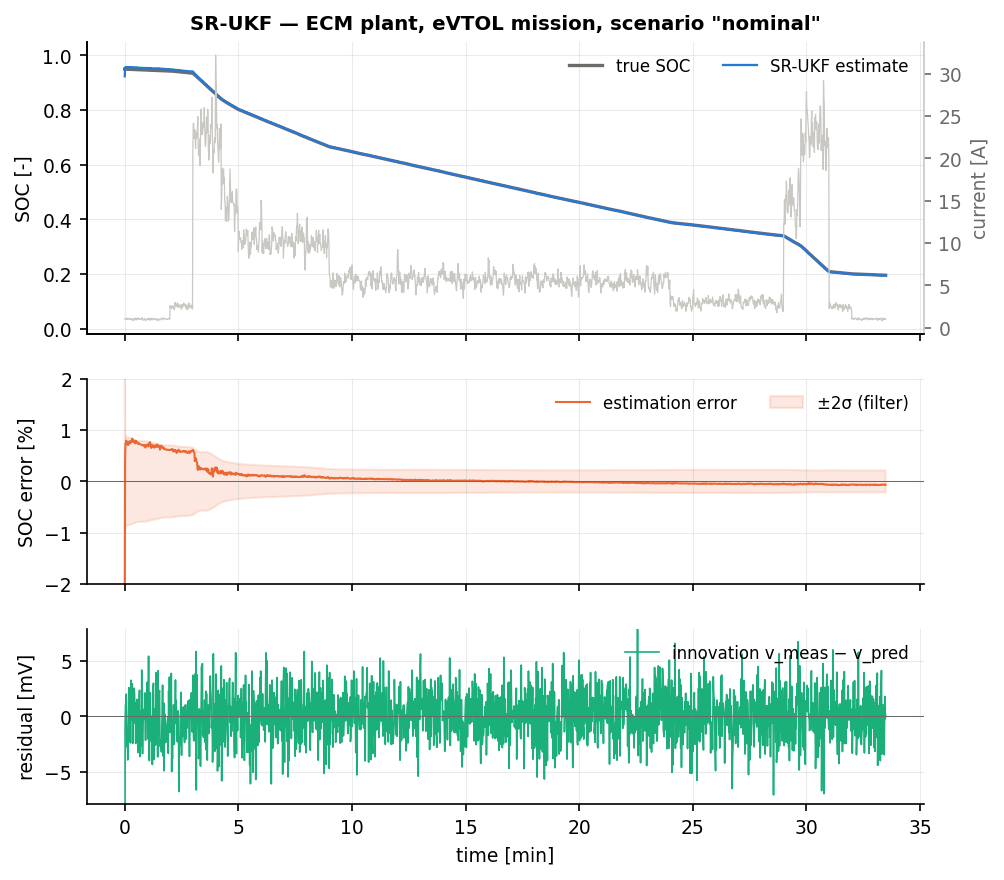
\includegraphics[width=\textwidth]{figures/cell_SRUKF_nominal.png}
\caption{SR-UKF on the nominal eVTOL mission: true and estimated SOC (top), estimation error with the $\pm 2\sigma$ band when available (middle), voltage residual (bottom).}
\end{figure}
\begin{figure}[H]\centering
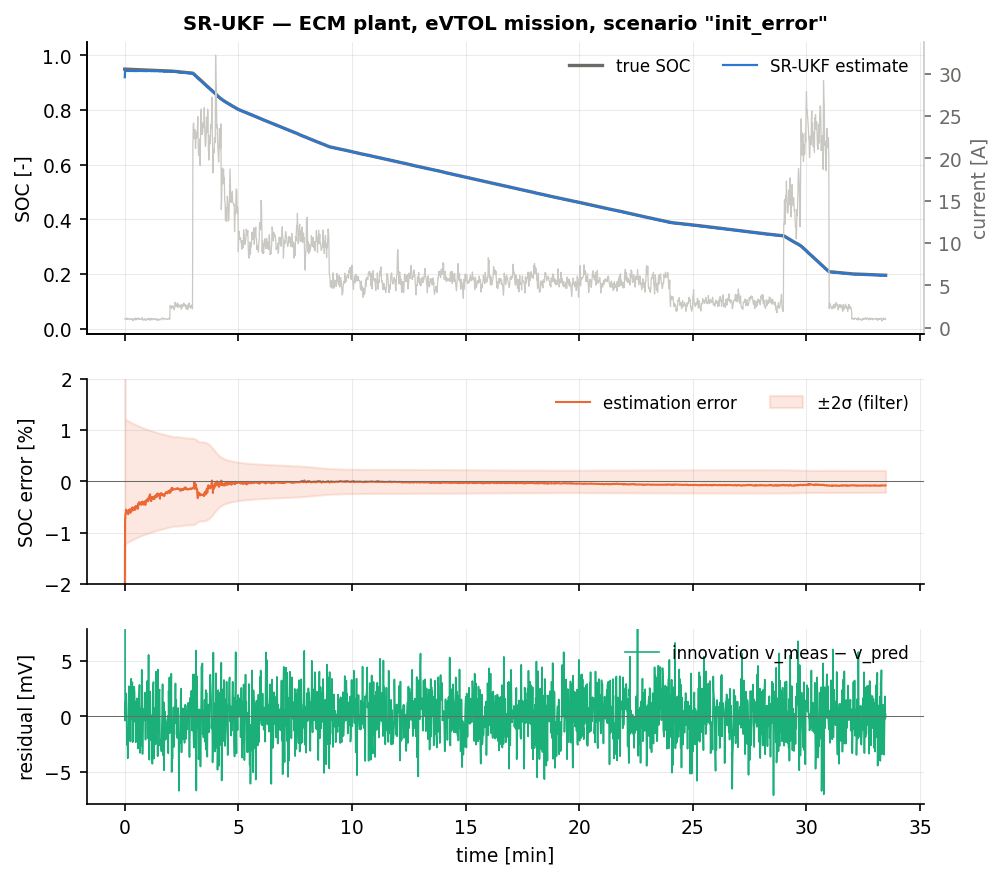
\includegraphics[width=\textwidth]{figures/cell_SRUKF_init_error.png}
\caption{SR-UKF with a 35\,\% initial SOC error.}
\end{figure}

All numbers are three-seed means in per cent SOC.

The SR-UKF reproduces the covariance UKF on all twelve ECM scenarios and all nine SPM scenarios
to two decimals: ECM \texttt{nominal} $0.20/0.04\,\%$, \texttt{init\_error} $0.17/0.07\,\%$
with $t_{\text{conv}} = 0$\,s, \texttt{current\_bias} $0.58/0.57\,\%$, \texttt{cold}
$0.27/0.07\,\%$, \texttt{aged\_cell} $1.10/1.36\,\%$, \texttt{param\_mismatch}
$1.29/1.37\,\%$, \texttt{sensor\_dropout} $1.39/0.86\,\%$, \texttt{preisach} $1.35/0.23\,\%$
($t_{\text{conv}} = 214$\,s), \texttt{combined} $1.23/1.19\,\%$ with $t_{\text{conv}} = 0$\,s.
Element-wise over a full mission the two agree to $\max\abs{\Delta\vx} = 4.1\times10^{-11}$ and
$\max\abs{\Delta\mP} = 2.3\times10^{-12}$ --- three orders of magnitude looser than the
SR-EKF/EKF agreement ($10^{-14}$), which is precisely the signature of the near-cancelling
downdate of Remark~\ref{rm:srukf-downdate}: about one significant digit is lost there, and the
remainder accumulates over $\num{18000}$ steps.

Like the UKF, the SR-UKF is the filter that survives \texttt{combined}: its steady-state
error of $1.19\,\%$ against the EKF's $12.44\,\%$ is the best figure of the fifteen on that
scenario. The reason is the one analysed in Chapter~\ref{ch:ukf}: its
predicted-measurement variance is inflated by the second-order term and the posterior does not
collapse after the first update. All other estimation behaviour --- the mild transient penalty
on \texttt{nominal}, the good \texttt{cold} and \texttt{aged\_cell} results, the degradation on
\texttt{sensor\_dropout} and the slow \texttt{preisach} convergence --- is that of
Chapter~\ref{ch:ukf}.

The cost conclusion differs from the SR-EKF's. There the factored form cost $70\,\%$ more time
for identical answers; here it costs $8\,\%$ ($1.42$--$1.57\,\SI{}{\micro\second}$ against the
covariance UKF's $1.34$--$1.46$), because the covariance UKF's two Cholesky factorisations per
step are exactly what the square-root form avoids. For that price it removes the failure mode
where a marginally indefinite $\mP$ stops the sigma-point generation.

The single-precision build is where this chapter's caveat earns its place. The
float-versus-double table shows the SR-UKF at $0.14\,\%$ on \texttt{nominal} in float32 against
$0.04\,\%$ in double --- a factor of $3.5$, and the largest nominal degradation of any filter in
this family, where the covariance UKF moves only from $0.04$ to $0.05\,\%$. That is the
rank-one downdate of \eqref{eq:srukf-mu2} cancelling $88\,\%$ of the pre-downdate variance
(Remark~\ref{rm:srukf-downdate}): in double the lost significant digit is invisible, in single
precision it is not. Nothing diverges, the errors remain far below the acceptance threshold, and
on the harder scenarios the float build is actually better ($0.96\,\%$ against $1.50\,\%$ on
\texttt{aged\_cell}, $0.23\,\%$ against $1.79\,\%$ on \texttt{combined}) --- but the nominal
number is a genuine warning. If the target is single precision and $\alpha$ must be small, use
$\lambda\ge0$ (see the discussion of the benchmark options above) or the cubature point set,
both of which make every rank-one modification an update rather than a downdate.

\paragraph{SPM plant: structured model error.}
\begin{figure}[H]\centering
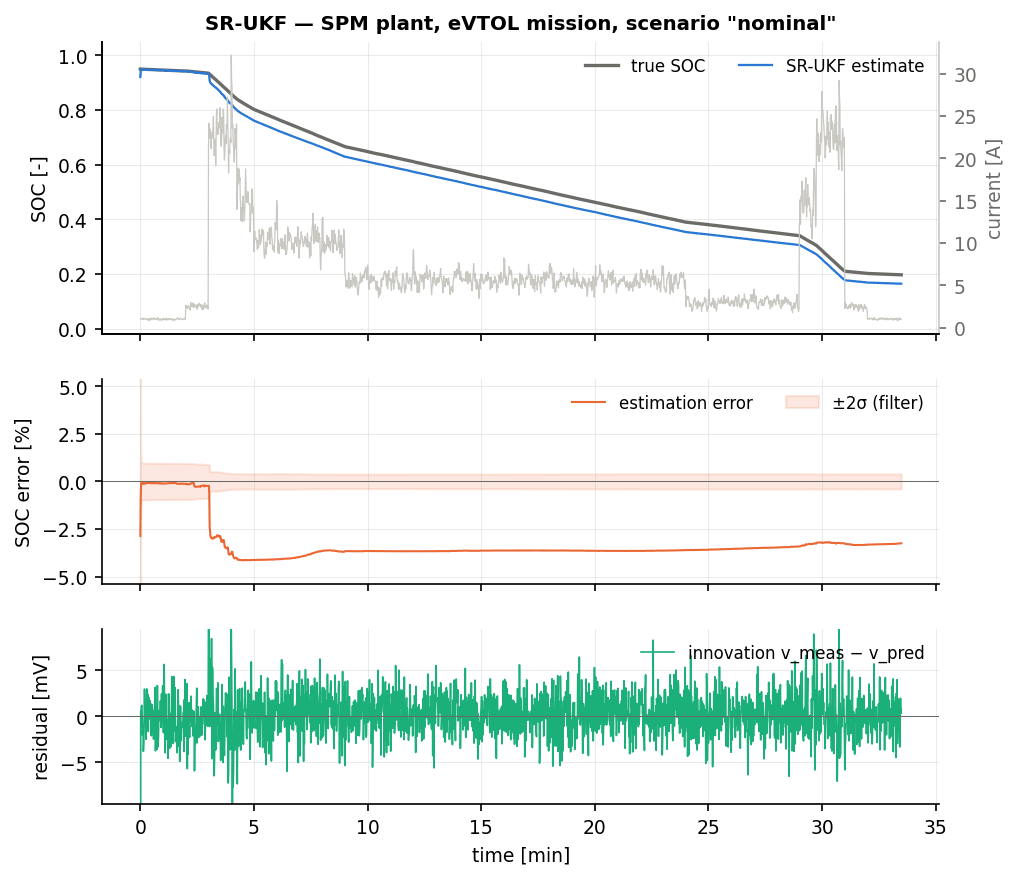
\includegraphics[width=\textwidth]{figures/cellspm_SRUKF_nominal.png}
\caption{SR-UKF on the nominal mission with the electrochemical (SPM) plant; identical to the covariance UKF.}
\end{figure}
The SPM block of the table is a different kind of test. The plant is the electrochemical
single-particle model; the estimator still runs a 2-RC equivalent circuit, fitted to that plant,
which leaves a \emph{structured} residual of about $4$\,mV (Butler--Volmer kinetics and
solid-phase diffusion that no 2-RC circuit can reproduce) and a slow second branch,
$\tau_2 = 556$\,s. Over a $33$-minute mission a $556$\,s pole barely relaxes, so $v_2(t)$ is
close to an affine ramp --- and so is $\ocv(\soc(t))$ while the cell discharges at a roughly
constant rate. The two channels through which the measurement sees the state,
$(\partial\ocv/\partial\soc)\,\delta\soc$ and $-\delta v_2$, are therefore nearly collinear in
the information accumulated over the flight: the pair $(\soc, v_2)$ is close to unobservable,
and no filter can decide whether a persistent few-millivolt residual belongs to the slow RC
branch or to the state of charge. Because that direction is weakly observable, a $4$\,mV
structured error maps onto \emph{several per cent} of SOC instead of the
$4\,\text{mV}/0.8\,\text{V}\approx0.5\,\%$ a well-conditioned channel would give. This
$(\soc,v_2)$ ambiguity, not the size of the residual, is the mechanism behind the
$3.7$--$4.6\,\%$ band in which the whole classical family sits.

The SR-UKF's SPM rows are the UKF's: $3.95/3.96\,\%$ on \texttt{nominal}, $8.29\,\%$ on
\texttt{cold}, $6.46\,\%$ on \texttt{current\_bias}, $7.26\,\%$ on \texttt{sensor\_dropout},
$4.95\,\%$ on \texttt{param\_mismatch}, $1.76\,\%$ on \texttt{outliers}. They sit slightly above
the EKF's ($3.73$, $7.35$, $5.69$, $5.31$, $3.13$, $1.99\,\%$), because a statistical
regression over the prior weights the ill-conditioned OCV channel more heavily than a tangent
does. Nothing diverges. It is worth noting for a square-root chapter that the SPM rows are the
only place in this report where the filters are visibly \emph{mis-specified}, and that the
covariance form remained positive definite there too: a structurally wrong model stresses the
estimator statistically, not numerically, so the factorisation neither helps nor hurts.

\section{Summary}
The square-root UKF is the form in which the unscented filter should be implemented: the same
estimates as the covariance UKF, guaranteed positive semi-definite $\mP$, no per-step
factorisation, and on this benchmark a time penalty of under $10\,\%$. The one caution --- and
the float results make it concrete --- is the rank-one downdate of the centre point, which with
a small $\alpha$ nearly cancels the QR result and costs roughly one significant digit,
visible as a $3.5\times$ nominal degradation in float32. A guarded implementation (fall-back
re-factorisation) makes this safe, and choosing $\lambda\ge0$ removes it entirely at the price
of a wider point spread.
